A crucial matter when designing a controller for automated operation of robotic surgery tools is the necessity of guaranteed patient safety. The system has to not only be able to prevent the surgery tool from entering certain regions, e.g. penetrating the wall of the heart or cutting an artery, but to guarantee that this cannot happen under any circumstances.

Casting the controller design problem as an optimization problem with constraints, such as e.g. \gls{mpc}, could in principle guarantee that the tool would not enter a predefined area, but a hard constraint would fail to follow the dynamics of a moving area boundary such as a beating heart.
Another and very elegant and computationally sound approach to the safe controller analysis and design problem is the use of barrier certificates, which provide a formal proof of safe operation \citep{bib:safety}. This chapter describes the requirements for the construction of barrier certificates along with notation used in relation to these.

%dealing with those topics within robotic surgeries feature necessary conditions to guarantee the patient safety and to avert patient trauma .





\section{Constraints for a Barrier Certificate}\label{sec:safety-def}

When a barrier certificate can be found for a (closed-loop) dynamical system, the controller is guaranteed to be safe. A general state-space representation of an $n$-dimensional non-linear system is considered:
\begin{flalign*}
\dot{x} = f_{cl}(x) + h(x)\,d = f(x) + g(x)\,u + h(x)\,d
\end{flalign*}
\begin{tabular}{rl} 
where &  \\
\gls{x} &  is the state, $x \in \mathbb{R}^n$\\
\gls{u} & is the control input, $u \in \mathbb{R}^m$\\
\gls{d} & is the disturbance input, $d \in D \subseteq \mathbb{R}^p$ \\
\gls{f} & is a non-linear function, $f:\mathbb{R}^n \rightarrow \mathbb{R}^n$\\
\gls{g} & is a non-linear function, $g:\mathbb{R}^n \rightarrow \mathbb{R}^{n \times m}$\\
\gls{h} & is a non-linear function, $h:\mathbb{R}^n \rightarrow \mathbb{R}^{n \times p}$
\end{tabular}\\

A barrier certificate is defined, and the safe controller valid, for a region of the state space $\mathcal{X} \subseteq \mathbb{R}^n$, with unsafe region $\mathcal{X}_u \subseteq \mathcal{X}$ and (safe) initial region $\mathcal{X}_0$. Now safety of the closed-loop control system $\Gamma_\text{cl} = (f_\text{cl},h,\mathcal{X},\mathcal{X}_0,\mathcal{X}_u,D)$ is given according to \citep{bib:safety} as:
%\begin{exa}

\begin{quotation}
\subsubsection*{Definition of a safe system}
$\Gamma_\text{cl}$ is unsafe if $\exists \, t \in [0,$\gls{T}$]$ such that the trajectory $\phi_{X_0}^{\bar{d}} : [0,T]$ satisfies
\begin{flalign}
\left( \phi_{\mathcal{X}_0}^{\bar{d}}([0,t]) \cap \mathcal{X}_u \right) \neq \emptyset \kk \wedge \kk 
\phi_{\mathcal{X}_0}^{\bar{d}}([0,t]) \subseteq \mathcal{X}
\label{eq:defsafety}
\end{flalign}
\noindent
$\Gamma_\text{cl}$ is safe if there are no unsafe trajectories.
\end{quotation}

%\vspace{-0.2cm}
%
%\begin{longtable}{p{.9\textwidth} p{.1\textwidth} p{.1\textwidth}} 
%Where  & & \\
%\gls{fcl} is a potential non-linear function with the closed loop characteristic:\\ \kk $f_\text{cl}: x \mapsto f(x)+g(x)k(x)$ where \gls{k} is the feedback gain with the map $k: \mathbb{R}^n \rightarrow \mathbb{R}^m$ & [$\cdot$] &  \\
%\gls{X} is the set of all allowed states & [$\cdot$] &  \\
%\gls{X0} is the set of all allowed initial states & [$\cdot$] &  \\
%\gls{Xu} is the set of all unsafe states & [$\cdot$] &  \\
%\gls{phi} is the set of all allowed initial conditions with the bounded disturbance input \gls{dbar} & [$\cdot$]
%\end{longtable}

Here \gls{phi} denote the trajectory of the system with initial state $x_0\in \mathcal{X}_0$ and bounded disturbance function $\bar{d}:\mathbb{R}_{\geq 0} \rightarrow D$. A graphical interpretation of \autoref{eq:defsafety} is shown in \autoref{fig:defsafety}.

\begin{figure}[H]
	\center
	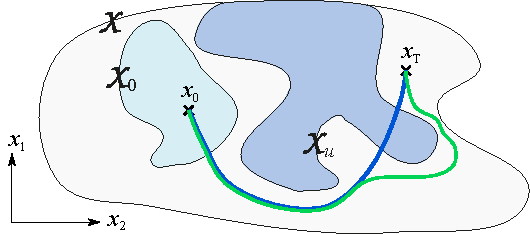
\includegraphics[width=0.6\textwidth]{safety.pdf}	
	\caption{Graphical interpretation of \autoref{eq:defsafety} in the state space. The blue trajectory is unsafe because $\left( \phi_{\mathcal{X}_0}^{\bar{d}}([0,t]) \cap \mathcal{X}_u \right) \neq \emptyset$, while the green trajectory is safe.}
	\label{fig:defsafety}
\end{figure}
\label{def_safety}
%\end{exa}


A closed-loop system is safe if a barrier certificate can be constructed as a function $B(x):\mathcal{X} \rightarrow \mathbb{R}$ adhering to the following constraints:
\begin{subequations}\label{eq:barrier_constraints}
\begin{flalign}
B(x) &\leq 0 \kk  \forall \hspace{2mm} x \in \mathcal{X}_0  \label{cer1}\\
B(x) &> 0  \kk  \forall \hspace{2mm} x \in \mathcal{X}_u \label{cer2} \\
L_{f_{cl}}B(x) &\leq 0 \kk  \forall \hspace{2mm} x \in \mathcal{X} \label{cer3}
\end{flalign}
\end{subequations}
Where \gls{lie}$(x)$ is the Lie derivative of \gls{bar} along the trajectory of $f(x)$. As it can be seen from \autoref{eq:barrier_constraints} the definition of a barrier certificate strongly resembles that of a Lyapunov function, and indeed the Lie derivative nonpositivity constraint is identical to the time derivative constraint to a Lyapunov function:
\begin{equation}
\dot{x}  = f(x) = \frac{\partial x}{\partial t} \qquad
\left\{ \begin{array}{r l l}
L_fB(x) \hspace*{-2mm}&= \tfrac{\partial B(x)}{\partial x} f(x) \hspace*{-2mm}&= \tfrac{\partial B(x)}{\partial x} \frac{\partial x}{\partial t}\\
\dot{V}(x) \hspace*{-2mm}&= \tfrac{\partial V(x)}{\partial t} \hspace*{-2mm}&= \tfrac{\partial V(x)}{\partial x}\tfrac{\partial x}{\partial t}
\end{array} \right. \label{eq:dBdt_dVdt}
\end{equation}

From \autoref{eq:barrier_constraints} it can be seen that the function $B(x)$ must be constructed such that its zero level set delimits and separates the safe and the unsafe regions, while the Lie derivative constraint imposes that the derivative $dB(x)/dx$ must have the opposite sign of the state derivative $dx/dt$ for any state within the region $\mathcal{X}$ where $B(x)$ is defined. Furthermore from \autoref{eq:dBdt_dVdt} it is deduced that a controller incorporating the barrier certificate in its design will ensure stability if $B(x)\rightarrow \infty$ for $x\rightarrow \pm\infty$.

Two approaches are used in the following: in \autoref{chap:cbf} the barrier certificate is constructed by hand, and a guaranteed safe controller is constructed according to the method in \cite{bib:org_control} and used in combination with a standard state space controller, while in \autoref{chap:putinar} a standard state space controller is constructed and its safety is then validated by constructing a barrier certificate using Putinar's Positivstellensatz.



%The design of a safe controller features the property that a supplied control signal ensures compliance of the definition described in \autoref{sec:safety-def}.







